%standalone document for pgf-umlcd
\documentclass{standalone}

\usepackage{pgf-umlcd}
\usetikzlibrary{arrows.meta}

\renewcommand{\umltextcolor}{black}
\renewcommand{\umldrawcolor}{teal}
\renewcommand{\umlfillcolor}{white}

\begin{document}

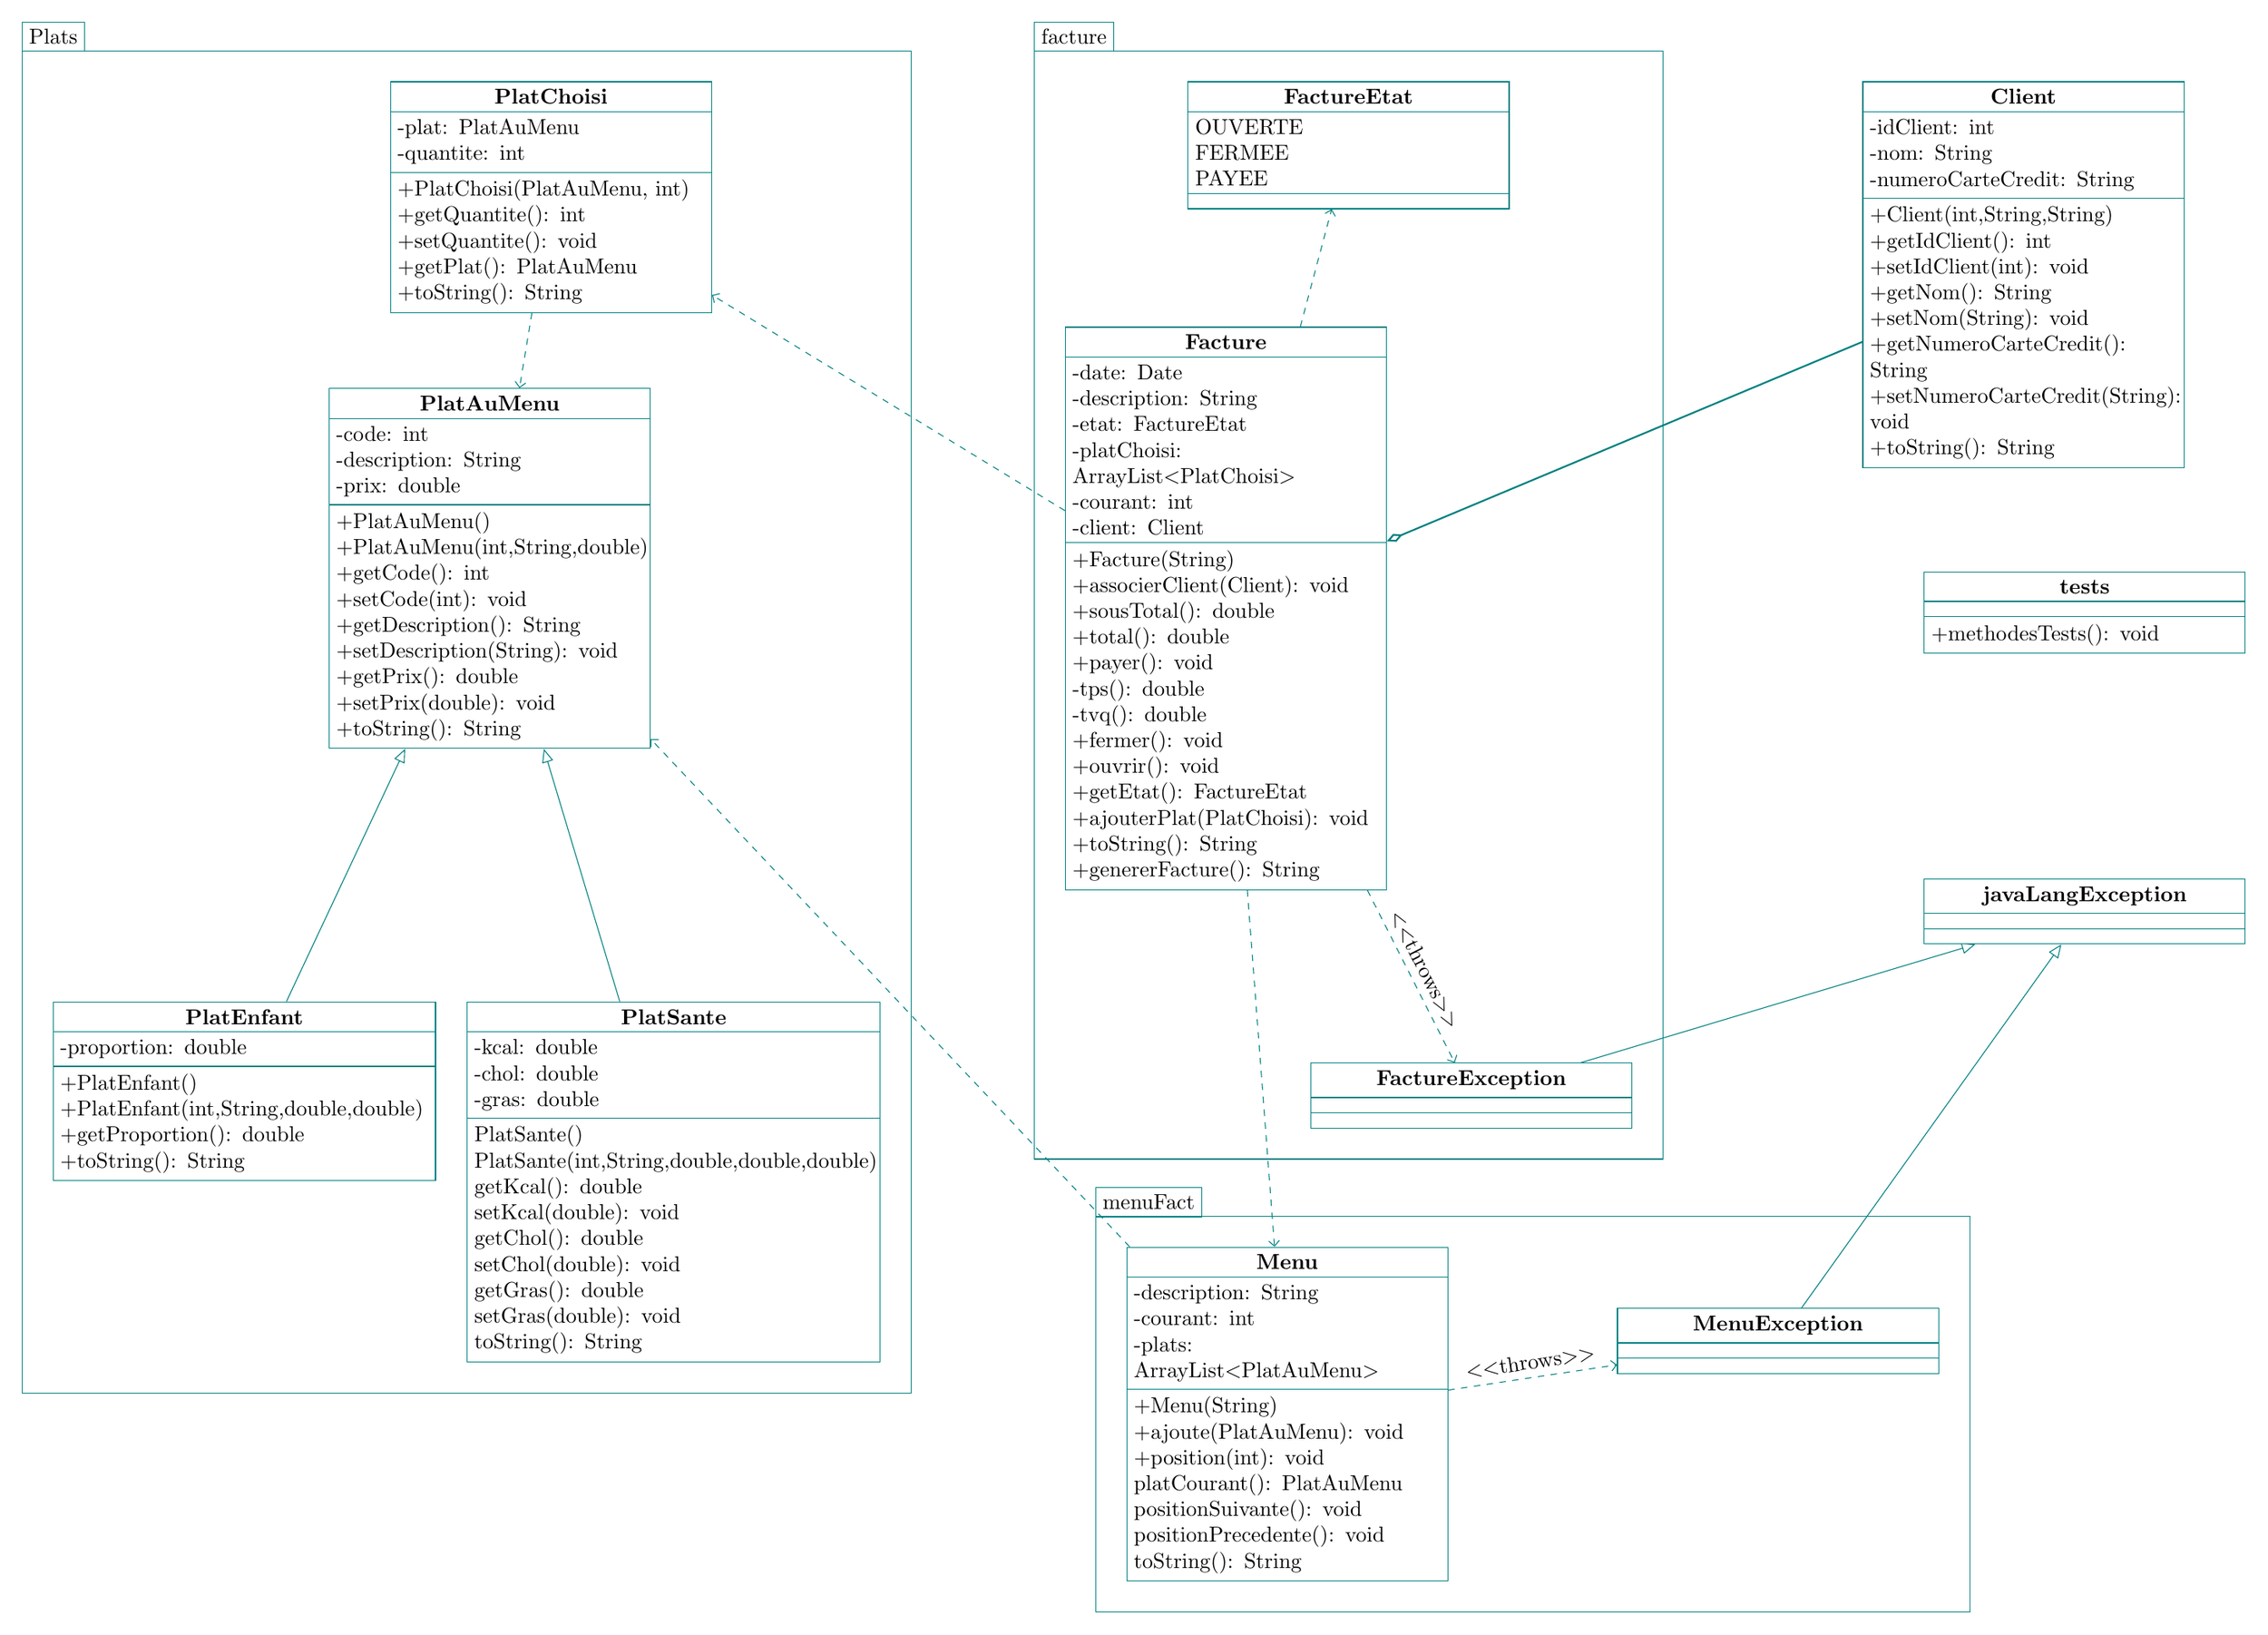
\begin{tikzpicture}

\begin{class}{Client}{24,0}
  \attribute{-idClient: int}
  \attribute{-nom: String}
  \attribute{-numeroCarteCredit: String}
  \operation{+Client(int,String,String)}
  \operation{+getIdClient(): int}
  \operation{+setIdClient(int): void}
  \operation{+getNom(): String}
  \operation{+setNom(String): void}
  \operation{+getNumeroCarteCredit(): String}
  \operation{+setNumeroCarteCredit(String): void}
  \operation{+toString(): String}
\end{class}{Client}{24,0}

\begin{class}{tests}{25,-8}
  \operation{+methodesTests(): void}
\end{class}{tests}

\begin{class}{javaLangException}{25,-13}
\end{class}

\begin{package}{Plats}

\begin{class}{PlatChoisi}{0,0}
  \attribute{-plat: PlatAuMenu}
  \attribute{-quantite: int}
  \operation{+PlatChoisi(PlatAuMenu, int)}
  \operation{+getQuantite(): int}
  \operation{+setQuantite(): void}
  \operation{+getPlat(): PlatAuMenu}
  \operation{+toString(): String}
  % \operation[0]{operation3()}
\end{class}

\begin{class}{PlatAuMenu}{-1,-5}
  \attribute{-code: int}
  \attribute{-description: String}
  \attribute{-prix: double}
  \operation{+PlatAuMenu()}
  \operation{+PlatAuMenu(int,String,double)}
  \operation{+getCode(): int}
  \operation{+setCode(int): void}
  \operation{+getDescription(): String}
  \operation{+setDescription(String): void}
  \operation{+getPrix(): double}
  \operation{+setPrix(double): void}
  \operation{+toString(): String}
  % Dotted arrow coming from PlatChoisi:
\end{class}

\begin{class}[text width=6cm]{PlatEnfant}{-5,-15}
  \inherit{PlatAuMenu}
  \attribute{-proportion: double}
  \operation{+PlatEnfant()}
  \operation{+PlatEnfant(int,String,double,double)}
  \operation{+getProportion(): double}
  \operation{+toString(): String}
\end{class}

\begin{class}[text width=6.5cm]{PlatSante}{2,-15}
  \inherit{PlatAuMenu}
  \attribute{-kcal: double}
  \attribute{-chol: double}
  \attribute{-gras: double}
  \operation{PlatSante()}
  \operation{PlatSante(int,String,double,double,double)}
  \operation{getKcal(): double}
  \operation{setKcal(double): void}
  \operation{getChol(): double}
  \operation{setChol(double): void}
  \operation{getGras(): double}
  \operation{setGras(double): void}
  \operation{toString(): String}
\end{class}

\end{package} % end of package "Plats"

\begin{package}{facture}

% TODO: Remove the empty methods section from this class
% TODO: figure out how to add the <<enum>> tag to FactureEtat
% \begin{class}{$<<$enum$>>$FactureEtat}{13,0}
\begin{class}{FactureEtat}{13,0}
  \attribute{OUVERTE}
  \attribute{FERMEE}
  \attribute{PAYEE}
\end{class}

\begin{class}{Facture}{11,-4}
  \attribute{-date: Date}
  \attribute{-description: String}
  \attribute{-etat: FactureEtat}
  % TODO: platChoisi has a typo in NDC. Make sure it's ok
  \attribute{-platChoisi: ArrayList$<$PlatChoisi$>$}
  \attribute{-courant: int}
  \attribute{-client: Client}
  \operation{+Facture(String)}
  \operation{+associerClient(Client): void}
  \operation{+sousTotal(): double}
  \operation{+total(): double}
  \operation{+payer(): void}
  \operation{-tps(): double}
  \operation{-tvq(): double}
  \operation{+fermer(): void}
  \operation{+ouvrir(): void}
  % TODO: getEtat has no () in NDC. Make sure it's ok
  \operation{+getEtat(): FactureEtat}
  % TODO: ajoutePlat has a typo in NDC. Make sure it's ok
  \operation{+ajouterPlat(PlatChoisi): void}
  \operation{+toString(): String}
  \operation{+genererFacture(): String}
\end{class}

\begin{class}{FactureException}{15,-16}
  \inherit{javaLangException}
\end{class}

\end{package} % end of package "facture"

\begin{package}{menuFact}

\begin{class}{Menu}{12,-19}
  \attribute{-description: String}
  \attribute{-courant: int}
  \attribute{-plats: ArrayList$<$PlatAuMenu$>$}
  \operation{+Menu(String)}
  \operation{+ajoute(PlatAuMenu): void}
  \operation{+position(int): void}
  \operation{platCourant(): PlatAuMenu}
  \operation{positionSuivante(): void}
  \operation{positionPrecedente(): void}
  \operation{toString(): String}
\end{class}

\begin{class}{MenuException}{20,-20}
  \inherit{javaLangException}
\end{class}

\end{package} % end of package "menuFact"


\draw[umlcd style dashed line,->] (PlatChoisi) -- (PlatAuMenu);
\draw[umlcd style dashed line,->]  (Facture) -- (FactureEtat);
\draw[umlcd style dashed line,->] (Facture) -- (Menu);
\draw[umlcd style dashed line,->] (Menu) -- (PlatAuMenu);
\draw[umlcd style dashed line,->] (Facture) -- (PlatChoisi);
\draw[umlcd style,thick, -{Diamond[open]}] (Client) -- (Facture);
\draw[umlcd style dashed line,->] (Facture) --node[above,sloped,black]{$<<$throws$>>$} (FactureException);
\draw[umlcd style dashed line,->] (Menu) --node[above,sloped,black]{$<<$throws$>>$} (MenuException);
\end{tikzpicture}

\end{document}


